% The "%" character denotes a comment
\documentclass[prb,preprint]{revtex4-1}
\usepackage{amsmath}  % needed for \tfrac, \bmatrix, etc.
\usepackage{amsfonts} % needed for bold Greek, Fraktur, and blackboard bold
\usepackage{graphicx} % needed for figures

\begin{document}
\title{PHYS 333 - Microprocessors Lab 03: PWM Outputs, Part II}
\author{Adam Stammer}
%\email{adam.stammer@go.winona.edu}

\date{\today}

%if you include an abstract, it goes here
\begin{abstract}
Pulse Width Modulation, turning a signal on and off as a means to control power, is used extensively as a more efficient alternative to using resistors to get a specified voltage. It's also used to vary power and voltage in a way that is difficult to do with resistors. That makes it a valuable tool in many Microprocessor projects, but sometimes we need a wave that isn't square and so it's important to know how to smooth that signal. In this lab we aimed to better understand and implement just that.
\end{abstract}

\maketitle
%title page ends here

\section{Notice}
Unfortunately I've switched to a new phone since doing the portion of this lab that I did accomplish. In the process I lost the majority of media relevant to this project. As such you won't find much for pictures or video as I lack the equipment to recreate them.


\section{Establishing a PWM Wave}
The first task was to create a PWM wave output. Since this was the only I/O for this system it was easy enough to achieve with simple delays. Turn the signal on, and wait for a fraction of the cycle time. Turn the signal off, and wait for the remainder of the cycle time. Repeat as necessary. Tweaking the duty cycle will change how the fractions of the cycle time are distributed. This was not new. You can see code for this below. Fig 1 shows a blurry example of the output.

\begin{verbatim}
int analogueWrite(float duty, long period, int pin) {
    digitalWrite(pin, HIGH);
    delayMicroseconds(duty*period);
    digitalWrite(pin, LOW);
    delayMicroseconds(period - (duty*period));
}
\end{verbatim}

\begin{figure}[ht]
	\centering
	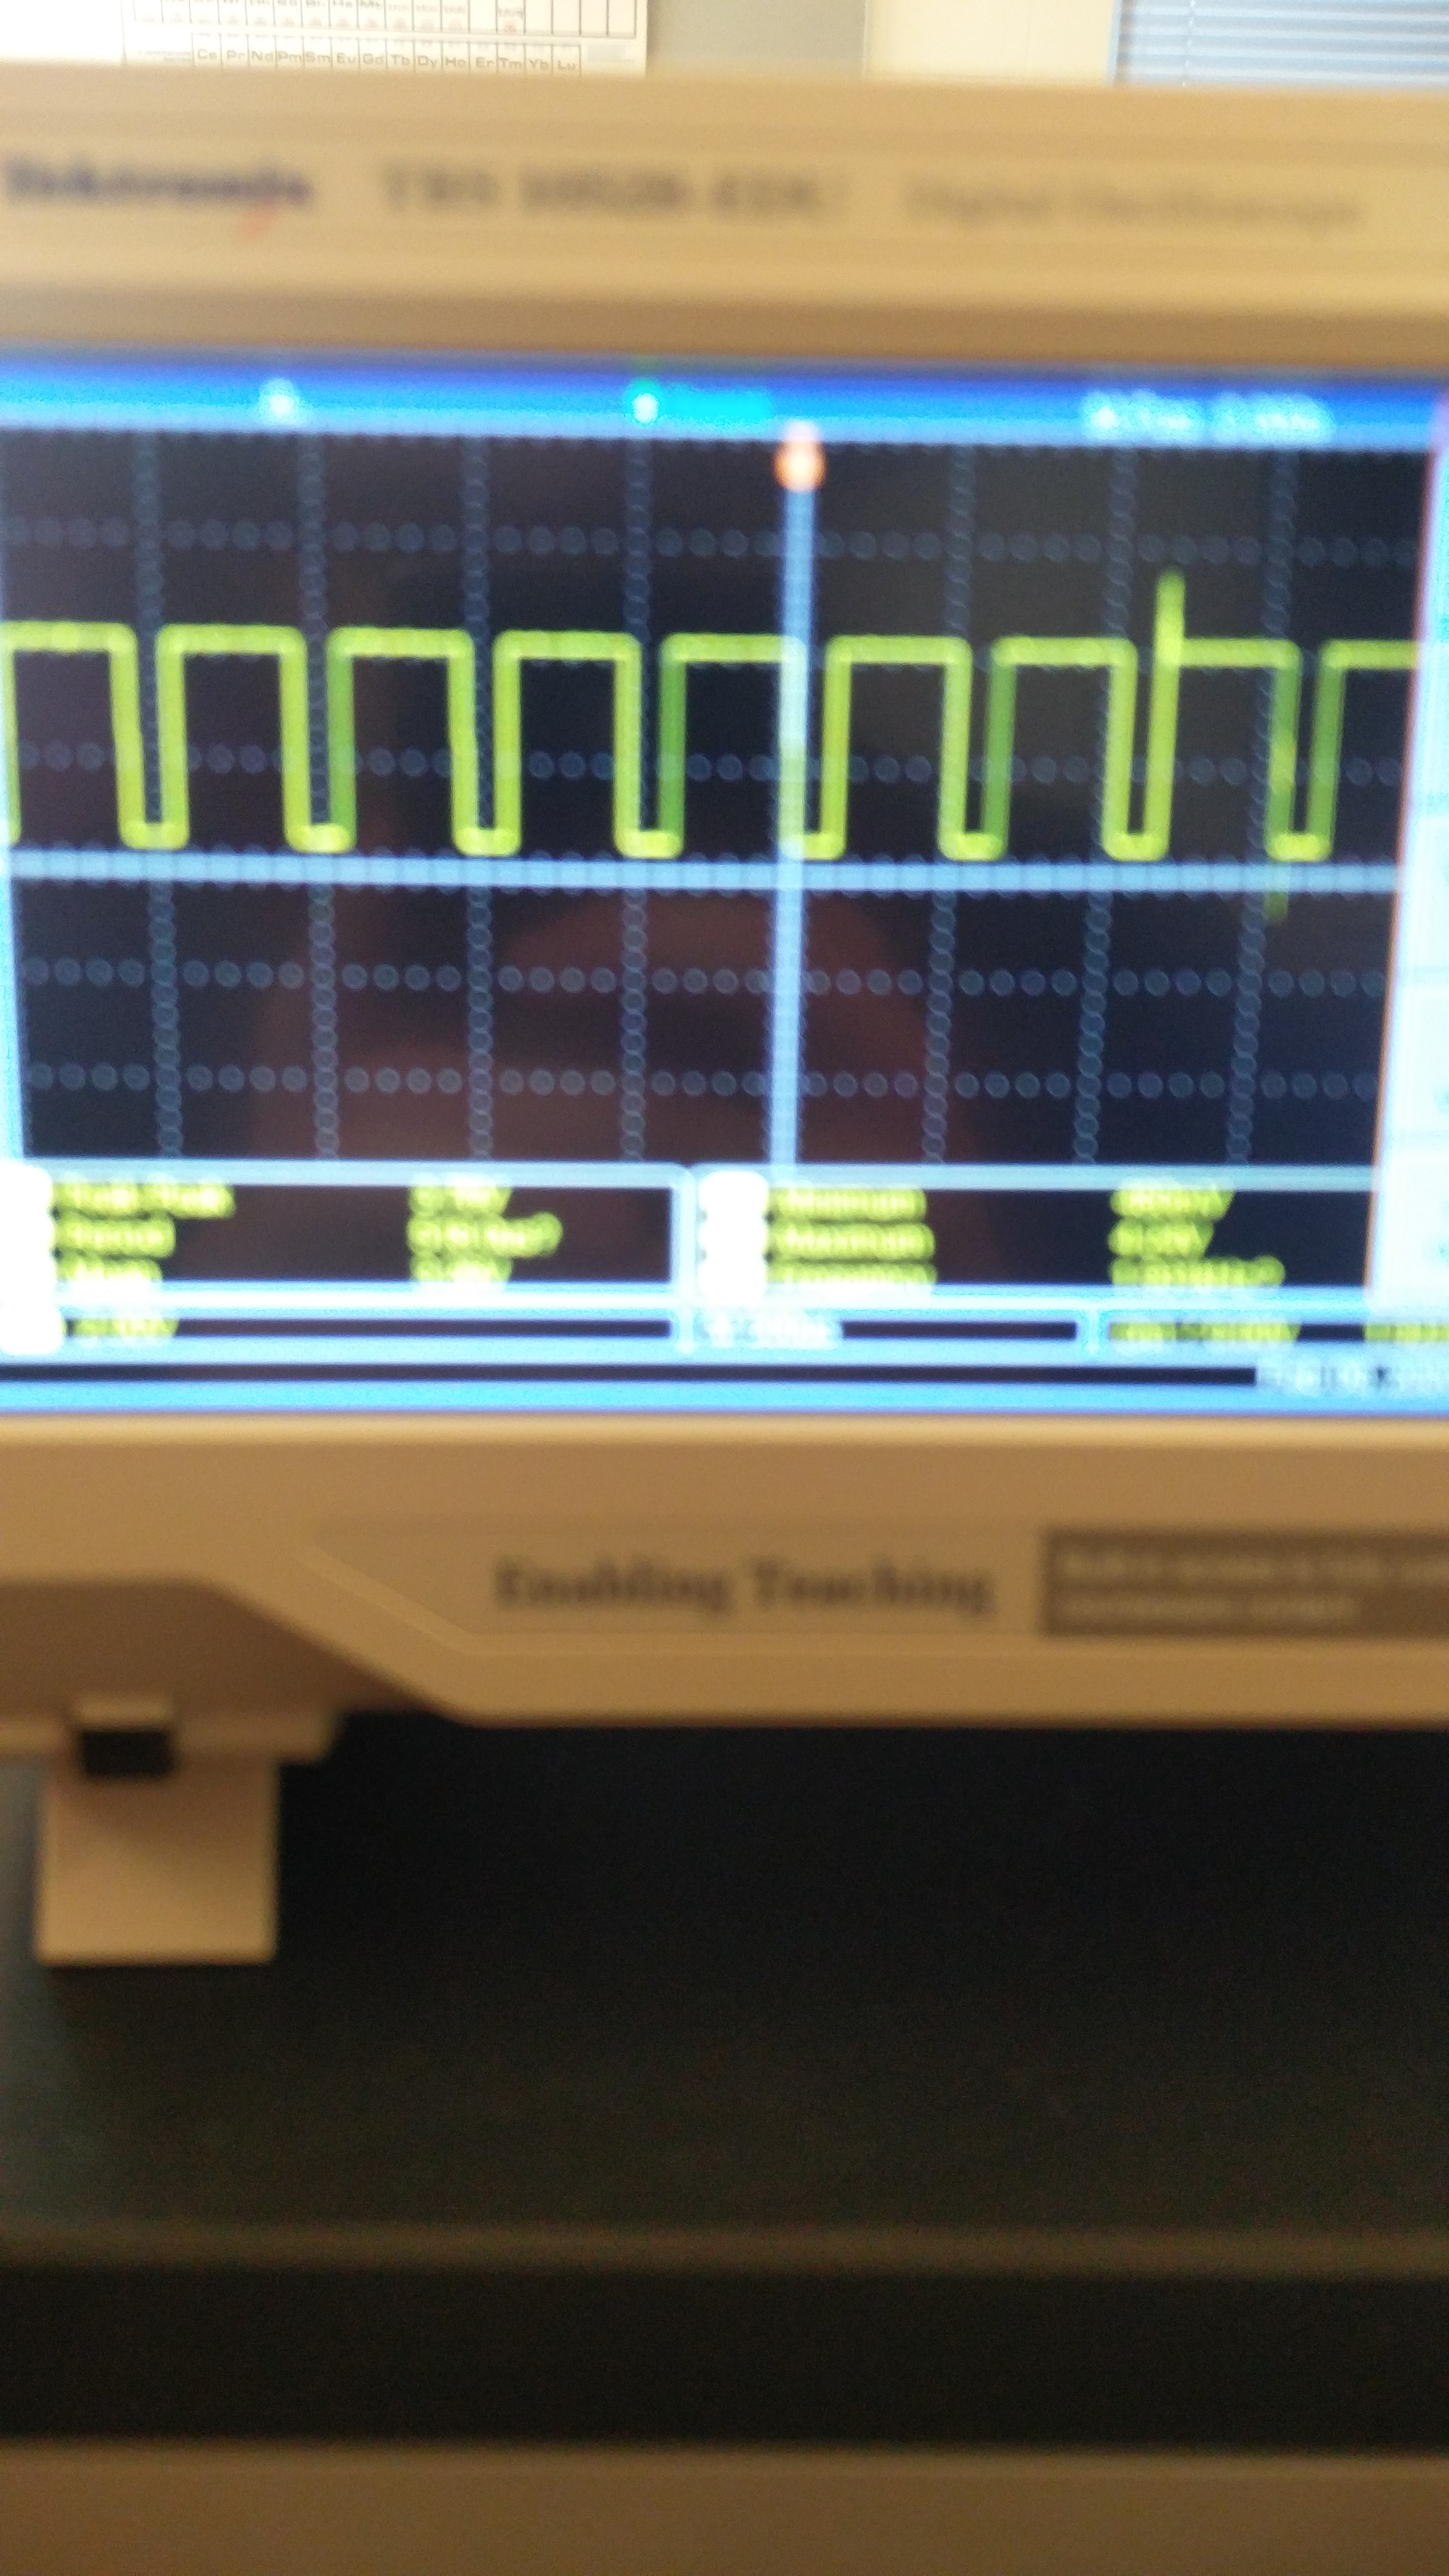
\includegraphics[width=4in]{square.jpg}
	\caption{Square Wave Output}
	\label{fig1}
\end{figure}


\section{The Second Section}
Now if we use the function above but change duty over time relative to a sin function, we can get a square output that grows in positive duty cycle before decrease and then growing again. I do not have a picture of this unfortunately. If we then take this output and filter it through a capacitor as described in the lab, we can smooth this signal out. You can look at some previous lab reports for more detail on this smoothing and the capacitor math involved. I just elected for a very large capacitor and hoped it would smooth it out enough, and it did.

At this point, the growing and shrinking duty cycle will charge the capacitor up over time before discharging it over time, also at the rate described by the sin wave. An example output of this can be seen below in Fig 2.

\begin{verbatim}
int analogueWriteSin(long cycle, int pin, int duration) {
    for(int i = 0; i < cycle; i++) {
        float f = i * 2* 3.14;
        analogueWrite((sin((f/cycle))+1.0)/2.0, cycle, pin);
    }
}
\end{verbatim}

\begin{figure}[ht]
	\centering
	\includegraphics[width=4in]{sin.jpg}
	\caption{Sin Wave Output}
	\label{fig1}
\end{figure}

\section{Song}
The next task was to turn this sin wave into a variable frequency output and use it to play a song. I though it would be fun to use something other than a speaker for this, so with the help of Robert, we managed to hook together a computer CPU cooler fan to a power supply and pipe our sin wave output to a transistor functioning as a digital on off switch. It kind of defeated the purpose of making it a sin wave, as most of our output was being turned right back into a square wave, but it was pretty cool. I can't currently find a video of it playing, but I believe we showed it to you. You can see the bulk of the code below.

Essentially, we converted each relevant note into a wave period. Then we converted the song "Take On Me" to notes and durations as described in the arrays at the head of the program. Then it was a simple matter of looping through the arrays and push the values to the output function.

\begin{verbatim}
int melody[] = {
    NOTE_FS5, NOTE_FS5, NOTE_D5, NOTE_B4, NOTE_B4, NOTE_E5, 
    NOTE_E5, NOTE_E5, NOTE_GS5, NOTE_GS5, NOTE_A5, NOTE_B5, 
    NOTE_A5, NOTE_A5, NOTE_A5, NOTE_E5, NOTE_D5, NOTE_FS5, 
    NOTE_FS5, NOTE_FS5, NOTE_E5, NOTE_E5, NOTE_FS5, NOTE_E5
};

// The note duration, 8 = 8th note, 4 = quarter note, etc.
int durations[] = {
    8, 8, 8, 4, 4, 4, 
    4, 5, 8, 8, 8, 8, 
    8, 8, 8, 4, 4, 4, 
    4, 5, 8, 8, 8, 8
};
// determine the length of the arrays to use in the loop iteration
int songLength = sizeof(melody)/sizeof(melody[0]);

void loop() {
    // Iterate through both arrays
    // The for loop stops when it is equal to the size of the melody array
    for (int thisNote = 0; thisNote < songLength; thisNote++){
        analogueWriteSin(200, 3, 1000);
    }
}
\end{verbatim}
%\begin{thebibliography}{99}
% The numeral (here 99) in curly braces is nominally the number of entries in
% the bibliography. It's supposed to affect the amount of space around the
% numerical labels, so only the number of digits should matter--and even that
% seems to make no discernible difference.
%Not Requested
%\end{thebibliography}

\end{document}
